
\section{Methodology}
In the evalutation below, we will use two sets of benchmarks:
\begin{enumerate}
\item \texttt{parallel-ml-bench}: an MPL-specific benchmark suite introduced as
  part of \citet{mpl-orig}. This benchmark suite is focused largely on
  parallelism-friendly workloads, i.e. HPC, computational geometry, etc.

\item The MLton benchmark suite: shipped as part of the MLton codebase, this
  benchmark suite captures only single-core performance, and emphasizes some
  more synthetic workloads to capture particular compiler capabilities (e.g. a
  comparison between tail-recursive and non-tail-recursive Fibonacci
  implementations).

\end{enumerate}

As we will see below, while the MLton benchmark suite does try to explicitly
cover array flattening, the workloads it exhibits seem to under-weight the
importance of the transformation.

All measurements were performed using the same compiler binary on both test
sides (MLton or MPL, respectively), using compiler flags to enable/disable
passes as needed to test the impact of each optimization. All ratios are
reported as \texttt{test / base}, i.e. <1.0 means ``smaller number on the test
side'' (the ``good'' outcome) and >1.0 means ``bigger number on the test side
(the ``bad'' outcome). Here \texttt{test} corresponds to the average across all
trials on the test side, and \texttt{base} corresponds to the average across all
trials on the base side. The number of trials is managed by the respective
benchmark frameworks in order to collect on the order of a few seconds of data
in each configuration.

All benchmarks use the C backend of MLton/MPL for codegen, calling into GCC
(version 15.2.0) to emit the final binary. We found that it was necessary to
compile the benchmarks under \texttt{-O2} (rather than the MLton default of
\texttt{-O1}) in order to obtain stable, interpretable performance data: with
\texttt{-O1}, we observed that the same compiler configuration would yield
dramatically different results on similar host CPUs (Intel Icelake vs AMD Ryzen
9), e.g. a 40\% slowdown on Intel vs a 10\% speedup on AMD. These differences
went away after supplying C compiler flags that controlled low-level code layout
options, e.g. \texttt{-falign-loops}. We also chose to enable
\texttt{-march=native} because it reduced the strange variance described above.

As we'll discuss in more detail below, directly examining the experiment data
makes it clear that trial runtimes are not normally distributed: as can be seen
examining \cref{fig:example_scatter_trials}, the measured runtimes often exhibit
a bimodal distribution, presumably related to the effect of the GC. As argued in
\citet{bootstrap-paper}, it is consequently incorrect to estimate uncertainty
using the standard deviation to construct a symmetric confidence interval --
instead, we (for the \texttt{parallel\_bench} suite) report 95\% confidence
intervals estimated using the bootstrap method.

The MLton benchmark framework does not report per-trial numbers, and so no
confidence intervals are included for the MLton data. Conversely, the parallel
ML bench framework does not measure compilation times, and so compilation time
impact is included only for MLton.

\begin{figure}[htbp]
  \centering
  \begin{subfigure}[b]{0.48\textwidth}
    \centering
    \includegraphics[width=\textwidth]{../analysis/charts/delunay_mlton_parallel_ml_bench_scatter.pdf}
    \caption{\texttt{delunay}}
    \label{fig:delunay_mlton_parallel_ml_bench_scatter}
  \end{subfigure}
  \hfill
  \begin{subfigure}[b]{0.48\textwidth}
    \centering
    \includegraphics[width=\textwidth]{../analysis/charts/dedup_mlton_parallel_ml_bench_scatter.pdf}
    \caption{\texttt{dedup}}
    \label{fig:dedup_mlton_parallel_ml_bench_scatter}
  \end{subfigure}
  \caption{Trial-by-trial execution time for two benchmarks (\texttt{delunay} and \texttt{dedup}) for the MLton compiler. The experimental side is the \texttt{tuple}-flattening configuration for \texttt{delunay} and \texttt{ConApp}-flattening for \texttt{dedup}.}
  \label{fig:example_scatter_trials}
\end{figure}


In order to more-faithfully measure cases where our optimizations impacted only
a small number of benchmarks (and to avoid including confusing noise in the
geomean results), we exclude cases where the optimization under test did not
change the generated code. In order to achieve bit-identical output binaries in
this case, it was necessary to:
\begin{itemize}

\item Pass \texttt{-link-opt -s} to strip debug info (otherwise the C compiler
  inserts strings into the binary that contain non-deterministic temporary
  filenames)

\item Manually override the ``magic number'' inserted by MLton into the
  generated binary to a fixed, deterministic value: this magic number is formed
  from hash of the compiler binary version (deterministic) and a call to
  \texttt{Random.word ()} (not necessarily fixed, in case the optimization pass
  advanced the state of the random number generator).

The purpose of this value is just to enable MLton to more easily correlate its
generated C code with the compiled binaries (for profiling and state
serialization), so our choice to hardcode \texttt{0x0} has no impact on
performance.

\end{itemize}

All of the benchmarks described below were run on \hl{TODO: DESCRIBE HW}

\hl{TODO: OUTLINE BENCHMARK SUITES, BENCHMARK HARDWARE}

\FloatBarrier
\section{Tuple Flattening}
For the evaluation below, we use the following configuration:
\begin{itemize}

\item \texttt{PreFlatten} runs after \texttt{Flatten} (in order to avoid
  introducing duplication in the case where the \texttt{Flatten} global analysis
  can already fix all callers)

\item \texttt{PreFlatten} only transforms non-tail-recursive functions

\item \texttt{PreFlatten} runs 10 ``recursive steps'' (\hl{TODO: EXPLAIN? REMOVE?}

\end{itemize}


\subsection{MLton benchmarks}
\hl{TODO: FORMATTING IS BAD, HOW TO CONDENSE?}

\begin{figure}[htbp]
  \centering
  \begin{subfigure}[b]{0.32\textwidth}
    \centering
    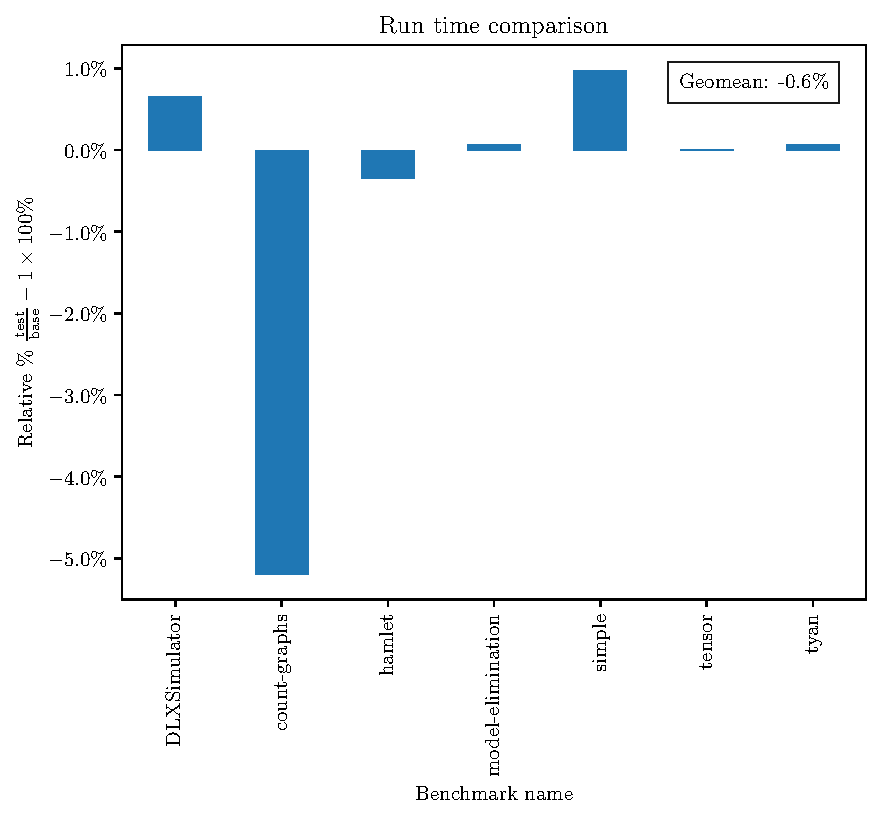
\includegraphics[width=\textwidth]{../analysis/charts/tuple_mlton_run_mlton_vs_mlton.pdf}
    \caption{Run time}
    \label{fig:tuple_mlton_run_mlton_vs_mlton}
  \end{subfigure}
  \hfill
  \begin{subfigure}[b]{0.32\textwidth}
    \centering
    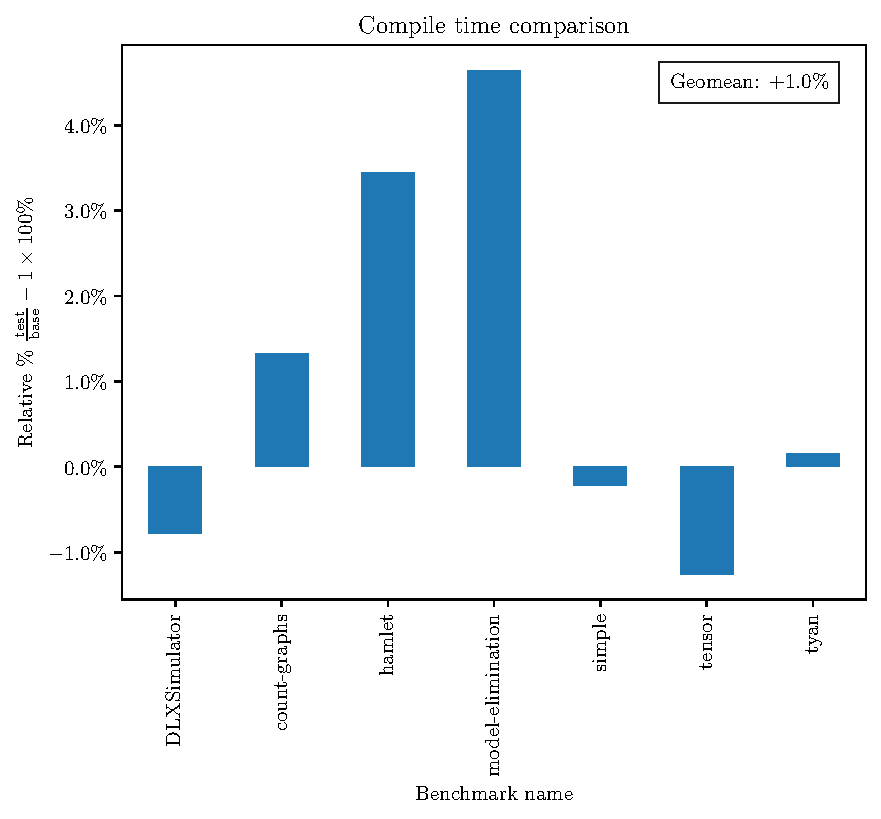
\includegraphics[width=\textwidth]{../analysis/charts/tuple_mlton_compile_mlton_vs_mlton.pdf}
    \caption{Compile time}
    \label{fig:tuple_mlton_compile_mlton_vs_mlton}
  \end{subfigure}
  \hfill
  \begin{subfigure}[b]{0.32\textwidth}
    \centering
    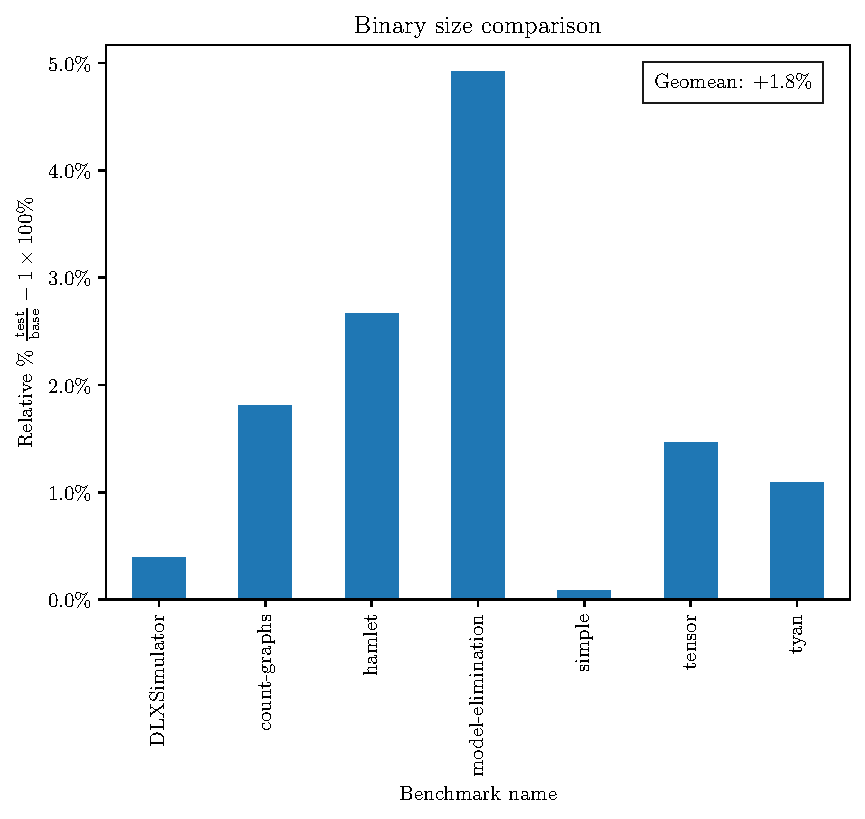
\includegraphics[width=\textwidth]{../analysis/charts/tuple_mlton_size_mlton_vs_mlton.pdf}
    \caption{Binary size}
    \label{fig:tuple_mlton_size_mlton_vs_mlton}
  \end{subfigure}
  \caption{Relative performance for with- vs without-\texttt{PreFlatten} on the MLton benchmark suite. <0\% represents an improvement, >0\% represents a regression.}
  \label{fig:tuple_mlton}
\end{figure}

As seen in \cref{fig:tuple_mlton}, the tuple flattning optimization is broadly
neutral for MLton on the MLton benchmark suite, with <5\% impact on all metrics.

\subsection{\texttt{parallel-ml-bench}: MLton vs MLton}

\begin{figure}[htbp]
  \centering
  \begin{subfigure}[b]{0.48\textwidth}
    \centering
    \includegraphics[width=\textwidth]{../analysis/charts/tuple_parallel_bench_run_mlton_vs_mlton.pdf}
    \caption{Run time}
    \label{fig:tuple_parallel_bench_run_mlton_vs_mlton}
  \end{subfigure}
  \hfill
  \begin{subfigure}[b]{0.48\textwidth}
    \centering
    \includegraphics[width=\textwidth]{../analysis/charts/tuple_parallel_bench_size_mlton_vs_mlton.pdf}
    \caption{Binary size}
    \label{fig:tuple_parallel_bench_size_mlton_vs_mlton}
  \end{subfigure}
  \caption{Relative performance for with- vs without-\texttt{PreFlatten}, applied to tuple constructors on the \texttt{parallel-ml-bench} benchmark suite. <0\% represents an improvement, >0\% represents a regression.}
  \label{fig:tuple_parallel_bench}
\end{figure}

As in the previous section, the impact of the tuple optimization on MLton for
parallel ML bench is also broadly neutral, as seen in
\cref{fig:tuple_parallel_bench}.

One exception is \texttt{reverb}, which shows a huge (40\%) confidence interval.
Examining the raw data in \cref{fig:reverb_tuple_scatter} makes it clear that
both the base and test sides exhibit extreme run-to-run variance (more than a
factor of 2) and so the noise is inherent to the benchmark rather than a new
effect of the tuple flattening optimzation.

\begin{figure}[htbp]
  \centering
  \includegraphics[width=\textwidth]{../analysis/charts/reverb_mlton_parallel_ml_bench_scatter.pdf}
  \caption{Trial-by-trial execution time for \texttt{reverb} in the \texttt{tuple}-flattening configuration.}
  \label{fig:reverb_tuple_scatter}
\end{figure}


\subsection{\texttt{parallel-ml-bench}: MPL vs MPL}

\begin{figure}[htbp]
  \centering
  \begin{subfigure}[b]{0.48\textwidth}
    \centering
    \includegraphics[width=\textwidth]{../analysis/charts/tuple_parallel_bench_run_mpl_vs_mpl_trellis.pdf}
    \caption{Run time}
    \label{fig:tuple_parallel_bench_run_mpl_vs_mpl}
  \end{subfigure}\hfill
  \begin{minipage}[b]{0.48\textwidth}
    \begin{subfigure}{\textwidth}
      \centering
      \includegraphics[width=\textwidth]{../analysis/charts/tuple_parallel_bench_run_mpl_vs_mpl_geomean.pdf}
      \caption{Geomean only}
      \label{fig:tuple_parallel_bench_geomean_mpl_vs_mpl}
    \end{subfigure}

    \begin{subfigure}{\textwidth}
      \centering
      \includegraphics[width=\textwidth]{../analysis/charts/tuple_parallel_bench_size_mpl_vs_mpl.pdf}
      \caption{Binary size}
      \label{fig:tuple_parallel_bench_size_mpl_vs_mpl}
    \end{subfigure}
  \end{minipage}
  \caption{Relative performance for with- vs without-\texttt{PreFlatten}, applied to tuple constructors on the \texttt{parallel-ml-bench} benchmark suite, for the MPL compiler, at a variety of core counts. <0\% represents an improvement, >0\% represents a regression.}
  \label{fig:tuple_parallel_bench_mpl}
\end{figure}

As we see in \cref{fig:tuple_parallel_bench_mpl}, the \texttt{tuple}
optimization has a mixed effect, with some benchmarks showing consistent wins
across core counts, and others showing losses. In order to further investigate
this effect, we'll select two representative benchmarks: \texttt{bfs} (a
consistent win) and \texttt{delaunay} (a consistent loss).

\subsection{\texttt{delaunay} vs \texttt{bfs}: observed IR change}

The \texttt{delaunay} benchmark solves the computational geometry problem of
\textit{Delaunay triangulation}, which partitions the convex hull of a set of
points into triangles whose smallest angles are maximal. In \texttt{delaunay},
the pass flattens arguments to 3 called functions (via duplication):

\begin{enumerate}
\item \texttt{flushArr}: part of the implementation of the \texttt{print} function
\item \texttt{makeTreeBounded}: part of the initialization logic, not included
  in the benchmarked region.
\item \texttt{parfor}: Transforms one branch of MPL's parallel \texttt{for} loop
  construct, going from:

\begin{minted}{python}
  # Parallel for loop on the range (lo, hi) with parallel grain size `grain`
  def parfor(f: 'a -> 'b, lo_hi: int * int, grain: int):
    (lo, hi) = lo_hi # unpack tuple
    # ...end conditions...
    # recursive spawn
    mid = lo + (hi - lo) / 2
    def left():
      parfor (f, (lo, mid), grain)
    def right():
      parfor (f, (mid, hi), grain)
    # launch left + right in parallel
    par (left, right)
\end{minted}
and flattening one of the two \texttt{parfor} recursive calls, i.e.:
\begin{minted}{python}
  # Parallel for loop on the range (lo, hi) with parallel grain size `grain`
  def parfor(f: 'a -> 'b, lo_hi: int * int, grain: int):
    (lo, hi) = lo_hi # unpack tuple
    # ...end conditions...
    # recursive spawn
    mid = lo + (hi - lo) / 2
    def left():
      parfor (f, (lo, mid), grain)
    def right():
      parfor_flat (f, mid, hi, grain)  # flattened recursive call
    # launch left + right in parallel
      par (left, right)

  # flattened specialization of `parfor`
  def parfor_flat(f: 'a -> b, lo: int, hi: int, grain: int): ...
    # ...end conditions...
    # recursive spawn
    mid = lo + (hi - lo) / 2
    def left():
      # construct tuple for unflattened call
      lohi = (lo, mid)
      parfor (f, lo_hi, grain)
    def right():
      parfor_flat (f, mid, hi, grain)  # flattened recursive call
    # launch left + right in parallel
    par (left, right)
\end{minted}
\end{enumerate}

Based on the action of the transformation, we would probably expect to see (for
\texttt{delaunay}):
\begin{enumerate}
\item A small win inside of \texttt{parfor} calls: while we could imagine the
  duplication adding some overhead due to instruction cache effects, the
  duplicated code is fairly small.

\item More-or-less no impact on any other part of the benchmark (test setup and
  \texttt{print} shouldn't have any impact on the per-trial runtime).
\end{enumerate}

%% Doing some arithmetic with the benchmark configuration, we can estimate on the
%% order of 500,000 calls to \texttt{parfor}, and so a $\approx 1$ \mu sec change
%% in this function's performance (which seems like a conservative upper bound for
%% the performance impact of the IR transformation above) should yield a change of
%% $\approx .5$ seconds of CPU time over the full benchmark (on the order of 7\%
%% out of the benchmark's full $\approx 7$ second runtime).

A savings materialized in \texttt{parfor} is consistent with what we see in the
benchmark: overhead in \texttt{parfor} adds delay in spwaning new tasks, and so
we would expect a larger savings at higher core counts. However, the consistent
loss at lower core counts is hard to explain on the basis of the observed IR
transformation.

In the \texttt{bfs} benchmark, the program calculates the BFS tree of an input
graph (i.e. the undirected distance between some distinguished source node and
all other nodes in the graph). The pass applies the following transformations to
\texttt{bfs}:
\begin{enumerate}
\item \texttt{parfor}: the same inline-the-right-hand-branch as above

\item \texttt{parVisitMany}: structurally identical to \texttt{parfor}, manages
  parallel fanout across graph nodes based on their indices

\item \texttt{sumOfOutDegrees}: avoids constructing a temporary tuple to pass as
  an argument to a paralllel reduce operation, roughly:

\begin{minted}{python}
  def sumOfOutDegrees(all_nodes: int array):
    def do_reduce(env: (...complex, 7-element tuple type...)):
      ... calculate sum ...
    reduce(do_reduce, all_nodes)
\end{minted}

where we flatten the \texttt{do\_reduce} call and avoid building the intermediate
\texttt{env} argument.

\end{enumerate}

These changes seem broadly consistent with the observed data, apart from the
observation that the win disappears at higher core counts: given the large error
bars, we can probably explain that effect as either pure noise, or changed GC
behavior (since GC pauses show up as outliers in the trial data).

Next, we'll dig into these results in more detail in order to further explain
the observed trends.


%% \hl{TODO: descibe that they change irrelevant portions}

\subsection{\texttt{delaunay} vs \texttt{bfs}: microarchitectural effects}
A first quick test is to run the microbenchmarks under \texttt{perf} and observe
what (if any) microarchitectural bottlenecks have shifted under the
transformation: did we introduce extra memory traffic, causing the workload to
become backend-bound? Did we introduce code bloat that caused the workload to
become backend bound? One standard methodology for analyzing CPU performance
counter events in order to draw these conflusions is the ``top-down'' method,
introduced by \citet{topdown-paper}, and now supported by the standard Linux
\texttt{perf} tool. The data in this section was collected by running:
\begin{minted}{bash}
  $ perf stat -dd -D $DELAY ... benchmark invocation...
\end{minted}
with the value \texttt{\$DELAY} manually adjusted in order to exclude benchmark
initialization.


Beginning with \texttt{delaunay}, we have, for a single core (in \cref{tab:perf_comparison_delaunay_1core}):
    \begin{table}[htbp]
      \centering
      \caption{Performance metric comparison on 1 core (Delaunay, 1 core)}
      \label{tab:perf_comparison_delaunay_1core}
      \begin{tabular}{lrrr}
        \toprule
        \textbf{Metric} & \textbf{Baseline} & \textbf{Test} & \textbf{Diff / Change} \\
        \midrule
        \multicolumn{4}{l}{\textit{Execution Overview}} \\
        \quad Task Clock (s)           & 148.68 s   & 159.66 s   & +7.39\%   \\
        \quad Instructions ($10^9$)    & 410.49 B   & 464.52 B   & +13.16\%  \\
        \quad IPC                      & 0.90       & 0.98       & +8.89\%   \\
        \midrule
        \multicolumn{4}{l}{\textit{Rates and Miss Percentages}} \\
        \quad Branch Miss Rate         & 2.6\%      & 2.6\%      & 0.0 pp    \\
        \quad L1 D-Cache Miss Rate     & 10.6\%     & 9.3\%      & -1.3 pp   \\
        \quad LLC Load Miss Rate       & 15.8\%     & 15.5\%     & -0.3 pp   \\
        \quad dTLB Load Miss Rate      & 2.3\%      & 2.0\%      & -0.3 pp   \\
        \midrule
        \multicolumn{4}{l}{\textit{Topdown L1 Metrics}} \\
        \quad Retiring                 & 0.9\%      & 1.0\%      & +0.1 pp   \\
        \quad Bad Speculation          & 97.3\%     & 97.3\%     & 0.0 pp    \\
        \quad Frontend Bound           & 0.0\%      & 0.0\%      & 0.0 pp    \\
        \quad Backend Bound            & 1.8\%      & 1.7\%      & -0.1 pp   \\
        \bottomrule
      \end{tabular}
    \end{table}
where \texttt{pp} indicates the absolute difference in percentage points.
Examining the same benchmark at 160 cores, we get (in \cref{tab:perf_comparison_delaunay_160cores}):
\begin{table}[htbp]
  \centering
  \caption{Performance metric comparison on 160 cores (Delaunay, 160 cores)}
  \label{tab:perf_comparison_delaunay_160cores}
  \begin{tabular}{lrrr}
    \toprule
    \textbf{Metric} & \textbf{Baseline} & \textbf{Test} & \textbf{Diff / Change} \\
    \midrule
    \multicolumn{4}{l}{\textit{Execution Overview}} \\
    \quad Task Clock (s)           & 427.34 s   & 423.15 s   & -0.98\%   \\
    \quad Instructions ($10^9$)    & 1024.59 B  & 1048.69 B  & +2.35\%   \\
    \quad IPC                      & 0.82       & 0.85       & +3.66\%   \\
    \midrule
    \multicolumn{4}{l}{\textit{Rates and Miss Percentages}} \\
    \quad Branch Miss Rate         & 0.7\%      & 0.8\%      & +0.1 pp   \\
    \quad L1 D-Cache Miss Rate     & 8.3\%      & 8.0\%      & -0.3 pp   \\
    \quad LLC Load Miss Rate       & 17.7\%     & 18.0\%     & +0.3 pp   \\
    \quad dTLB Load Miss Rate      & 0.6\%      & 0.6\%      & 0.0 pp    \\
    \midrule
    \multicolumn{4}{l}{\textit{Topdown L1 Metrics}} \\
    \quad Retiring                 & 9.6\%      & 11.3\%     & +1.7 pp   \\
    \quad Bad Speculation          & 60.0\%     & 58.5\%     & -1.5 pp   \\
    \quad Frontend Bound           & 8.1\%      & 8.8\%      & +0.7 pp   \\
    \quad Backend Bound            & 22.3\%     & 21.4\%     & -0.9 pp   \\
    \bottomrule
  \end{tabular}
\end{table}
This allows us to draw the following conclusions:
\begin{itemize}
\item On an instruction-for-instruction basis, the \texttt{tuple} transformation
  increases efficiency: both instructions per cycle and the fraction of retiring
  instructions increase between the base and test side.
\item The \texttt{tuple} transformation increases the total instruction count
  required to complete the benchmark by a sufficiently-large amount to balance
  out the IPC improvement (for 1 core).
\item Single-threaded performance is dominated by branch predictor effects, with
  a shocking 97\% of utilization lost to bad speculation. At the full core
  count, the bottleneck shifts towards memory, with a larger fraction of CPU
  time spent waiting on memory (the ``backend bound'' increase).
\item \hl{TODO: MISS RATE METRICS?}
\end{itemize}

Next, for \texttt{bfs}, at one core we have (in \cref{tab:perf_comparison_bfs_1core}):
\begin{table}[htbp]
  \centering
  \caption{Performance metric comparison on 1 core (BFS, 1 core)}
  \label{tab:perf_comparison_bfs_1core}
  \begin{tabular}{lrrr}
    \toprule
    \textbf{Metric} & \textbf{Baseline} & \textbf{Test} & \textbf{Diff / Change} \\
    \midrule
    \multicolumn{4}{l}{\textit{Execution Overview}} \\
    \quad Task Clock (s)           & 172.59 s   & 164.21 s   & -4.86\%   \\
    \quad Instructions ($10^9$)    & 320.10 B   & 326.58 B   & +2.03\%   \\
    \quad IPC                      & 0.62       & 0.67       & +8.06\%   \\
    \midrule
    \multicolumn{4}{l}{\textit{Rates and Miss Percentages}} \\
    \quad Branch Miss Rate         & 1.4\%      & 1.4\%      & 0.0 pp    \\
    \quad L1 D-Cache Miss Rate     & 8.6\%      & 8.7\%      & +0.1 pp   \\
    \quad LLC Load Miss Rate       & 51.3\%     & 51.0\%     & -0.3 pp   \\
    \quad dTLB Load Miss Rate      & 2.7\%      & 2.8\%      & +0.1 pp   \\
    \midrule
    \multicolumn{4}{l}{\textit{Topdown L1 Metrics}} \\
    \quad Retiring                 & 1.1\%      & 1.2\%      & +0.1 pp   \\
    \quad Bad Speculation          & 90.9\%     & 90.3\%     & -0.6 pp   \\
    \quad Frontend Bound           & 0.0\%      & 0.0\%      & 0.0 pp    \\
    \quad Backend Bound            & 7.9\%      & 8.5\%      & +0.6 pp   \\
    \bottomrule
  \end{tabular}
\end{table}
and at 160 cores (in \cref{tab:perf_comparison_bfs_160cores}):
\begin{table}[htbp]
  \centering
  \caption{Performance metric comparison on 160 cores (BFS, 160 cores)}
  \label{tab:perf_comparison_bfs_160cores}
  \begin{tabular}{lrrr}
    \toprule
    \textbf{Metric} & \textbf{Baseline} & \textbf{Test} & \textbf{Diff / Change} \\
    \midrule
    \multicolumn{4}{l}{\textit{Execution Overview}} \\
    \quad Task Clock (s)           & 822.65 s   & 816.26 s   & -0.78\%   \\
    \quad Instructions ($10^9$)    & 1454.22 B  & 1423.12 B  & -2.14\%   \\
    \quad IPC                      & 0.61       & 0.60       & -1.64\%   \\
    \midrule
    \multicolumn{4}{l}{\textit{Rates and Miss Percentages}} \\
    \quad Branch Miss Rate         & 0.6\%      & 0.7\%      & +0.1 pp   \\
    \quad L1 D-Cache Miss Rate     & 7.8\%      & 8.0\%      & +0.2 pp   \\
    \quad LLC Load Miss Rate       & 44.6\%     & 44.7\%     & +0.1 pp   \\
    \quad dTLB Load Miss Rate      & 1.2\%      & 1.3\%      & +0.1 pp   \\
    \midrule
    \multicolumn{4}{l}{\textit{Topdown L1 Metrics}} \\
    \quad Retiring                 & 3.3\%      & 3.0\%      & -0.3 pp   \\
    \quad Bad Speculation          & 77.0\%     & 79.7\%     & +2.7 pp   \\
    \quad Frontend Bound           & 1.2\%      & 1.2\%      & 0.0 pp    \\
    \quad Backend Bound            & 18.6\%     & 16.1\%     & -2.5 pp   \\
    \bottomrule
  \end{tabular}
\end{table}
Here, we can see:
\begin{itemize}
\item While we still have instruction bloat, the increase to IPC / retiring
  pipeline slots was large enough to improve performance overall (showing as a
  decrease in ``Task Clock'').
\item This benchmark still suffers from extreme utilization loss due to bad speculation.
\item \hl{TODO: miss rates?}
\end{itemize}

On the whole, the microarchitectural data is not particularly enlightening in
terms of understanding the output of the \texttt{tuple} transformation: the main
interesting finding here is that the generated code evidently interacts
extremely poorly with the CPU's branch predictor.

Briefly examining the poor branch predictor behavior: one potential hypothesis
is that the observed behavior is the result of the heavy use of the jump table
structure of the generated C code described above. We can drill down into this
further by examinining the types of mispredicted branches: conditional
(taken/not-taken) vs indirect. If the high mispredict rate is a consequence of
the jump table structure in the emitted C, we would expect to see it manifest as
a high mispredict rate for indirect branches. If, on the other hand, the high
mispredict rate is simply a property of how the algorithm operates on the input
data, we would expect to see a high rate of mispredictions for conditional
branches.

Measuring using the lower-level \texttt{perf} events, we get the following data
(in \cref{tab:badspec_hierarchical_tuple}):
\begin{table}[htbp]
  \centering
  \caption{Branch mispredictions breakdown as a percentage of total mispredictions, for the \texttt{tuple} configuration.}
  \label{tab:badspec_hierarchical_tuple}
  \begin{tabular}{lrr}
    \toprule
    \textbf{Branch Type} & \textbf{Delaunay (1 core)} & \textbf{BFS (1 core)} \\
    \midrule
    \textbf{Conditional (Total)} & \textbf{95.32\%} & \textbf{99.87\%} \\
    \quad Taken                  & 52.41\%          & 48.45\%          \\
    \quad Not-taken              & 42.91\%          & 51.42\%          \\
    \textbf{Indirect}            &  \textbf{4.64\%} &  \textbf{0.06\%} \\
    \textbf{Return (\texttt{ret})}& \textbf{0.04\%} &  \textbf{0.08\%} \\
    \bottomrule
  \end{tabular}
\end{table}
Given that nearly all mispredictions are conditional rather than indirect, we
can conclude that the high mispredict rate is an inherent property of the
algorithm and the input data rather than a deficiency of MLton codegen.


\subsection{\texttt{delaunay} vs \texttt{bfs}: control for known effects}
Another strategy we can use to understand how the pass impacted performance
(trying to compensate for the lack of source-level profiling with MPL that we
might use to understand performance in another language) is to try to separate
out the actual intended change implemented by the pass (as described above) from
other downstream effects.

Digging more deeply into the action of the pass, we can identify three direct
consequences:
\begin{enumerate}
\item The actual function duplication/tuple-flattening change (described above).

\item The post-change IR cleanup, running the generic MLton \texttt{Simplify}
  pass to perform optimizations after flattening: perhaps the \texttt{tuple}
  optimization itself is unhelpful, and the win is just from running
  \texttt{Simplify} again. We can control for this by running \texttt{Simplify}
  on both the baseline and the test.

\item Later on, during the \texttt{Chunkify} pass, introducing the new,
  flattened functions: perhaps the \texttt{tuple} optimization's change to tuple
  layout has no direct impact, but the new functions happen to move around chunk
  boundaries in a way that is helpful/unhelpful. We can control for this by
  using the compiler flag \texttt{-chunkify one} to force all functions into a
  single C chunk (improving performance at the cost of C compile time).

\end{enumerate}

In \cref{fig:tuple_standouts_only}, we see the impact of these three different
configurations: the relative performance when enabling ``baseline fixup'' is
generally the same as our standard experimental configuration, the performance
under \texttt{-chunkify one} is virtually identical between the baseline and the
test.

Therefore, on these two benchmarks, the actual transformation of the pass has
nearly zero impact on performance: the most important driver of performance
changes is simply the accidental permutation of chunk boundaries by creating new
functions. Looking at a comparison of the geomeans across all benchmarks in
\cref{fig:tuple_exp_geomeans} broadly confirms that this observation holds
across the entire benhcmark suite, showing roughly identical performance between
the regular configuration and the with-baseline-fixup configuration, and
neutral-to-positive impact from tuple flattening.

See the full set of benchmark data for \texttt{-chunkify one} in
\cref{fig:tuple_all_chunkify_one}. This data indicates that while the
transformation does appear to have a significant impact on a handful of
benchmarks (\texttt{ocaml-lu-decomp}, \texttt{tokens}), it is otherwise
neutral-to-positive, with an impact of $< 2\%$ on performance in most cases.


\begin{figure}[htbp]
  \centering
  \begin{subfigure}[b]{0.48\textwidth}
    \centering
    \includegraphics[width=\textwidth]{../analysis/charts/tuple_exp_bfs.pdf}
    \caption{\texttt{bfs}}
    \label{fig:tuple_exp_bfs}
  \end{subfigure}
  \hfill
  \begin{subfigure}[b]{0.48\textwidth}
    \centering
    \includegraphics[width=\textwidth]{../analysis/charts/tuple_exp_delaunay.pdf}
    \caption{\texttt{delaunay}}
    \label{fig:tuple_exp_delaunay}
  \end{subfigure}
  \caption{Comparison of speedups across core counts for \texttt{bfs} and \texttt{delaunay} under three configurations: baseline tuple-vs-tuple, baseline with fixup, and with \texttt{-chunkify one}. <0\% represents an improvement, >0\% represents a regression.}
  \label{fig:tuple_standouts_only}
\end{figure}

\begin{figure}[htbp]
  \centering
  \includegraphics[width=\textwidth]{../analysis/charts/tuple_exp_geomeans.pdf}
  \caption{Comparison of geometric mean speedups across core counts for the baseline tuple configuration, baseline with fixup, and with \texttt{-chunkify one}. <0\% represents an improvement, >0\% represents a regression.}
  \label{fig:tuple_exp_geomeans}
\end{figure}

\begin{figure}[htbp]
  \centering
  \includegraphics[width=\textwidth,height=0.88\textheight,keepaspectratio]{../analysis/charts/tuple_chunkify_one_parallel_bench_run_mpl_vs_mpl_trellis.pdf}
  \caption{Relative performance for tuple flattening with \texttt{-chunkify one} on the \texttt{parallel-ml-bench} benchmark suite, for the MPL compiler, across core counts. <0\% represents an improvement, >0\% represents a regression.}
  \label{fig:tuple_all_chunkify_one}
\end{figure}

%% \hl{TODO: Look at output from chunkify one. Conclude that chunkify is the
%%   culprit. Link to an appendix with the full table of results from these
%%   experiments and conclude that there are more unexplained effects}.

%% As seen in \cref{fig:tuple_parallel_bench_mpl}, the \texttt{tuple} optimization
%% is a fairly consistent loss across the benchmark suite; with the most striking
%% example \texttt{dense-matmul} displaying a 30\% loss for lower core count tests.

%% \hl{TODO: NEED ANALYSIS. MAYBE HYPERTHREADING IS RELEVANT?}

\FloatBarrier
\section{\texttt{ConApp} Flattening}

For the evaluation below, we use the following configuration:

\begin{itemize}
\item \texttt{PreFlatten} runs before \texttt{Flatten} (so that \texttt{Flatten}
  has the chance to optimize away the tuples that remain after eliding the ADT
  tags)

\item \texttt{PreFlatten} transforms all functions (both tail-recurisve and not)

\item \texttt{PreFlatten} runs 10 ``recurisve steps'' (\hl{TODO: LIKE ABOVE?})
\end{itemize}

\subsection{MLton Benchmarks}

\begin{figure}[htbp]
  \centering
  \begin{subfigure}[b]{0.32\textwidth}
    \centering
    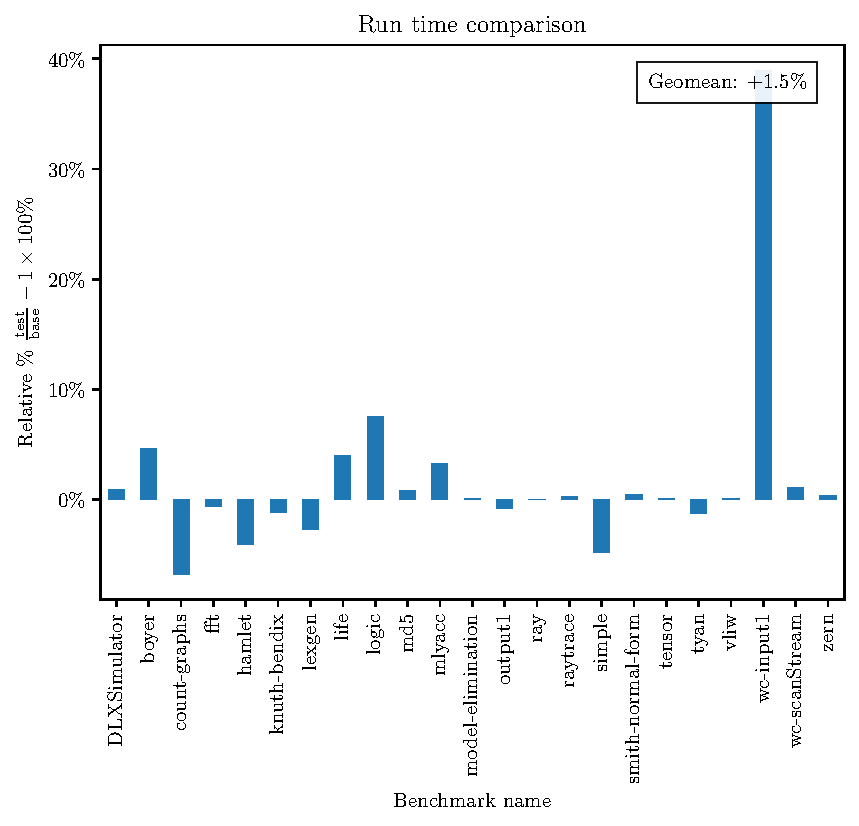
\includegraphics[width=\textwidth]{../analysis/charts/con_mlton_run_mlton_vs_mlton.pdf}
    \caption{Run time}
    \label{fig:con_mlton_run_mlton_vs_mlton}
  \end{subfigure}
  \hfill
  \begin{subfigure}[b]{0.32\textwidth}
    \centering
    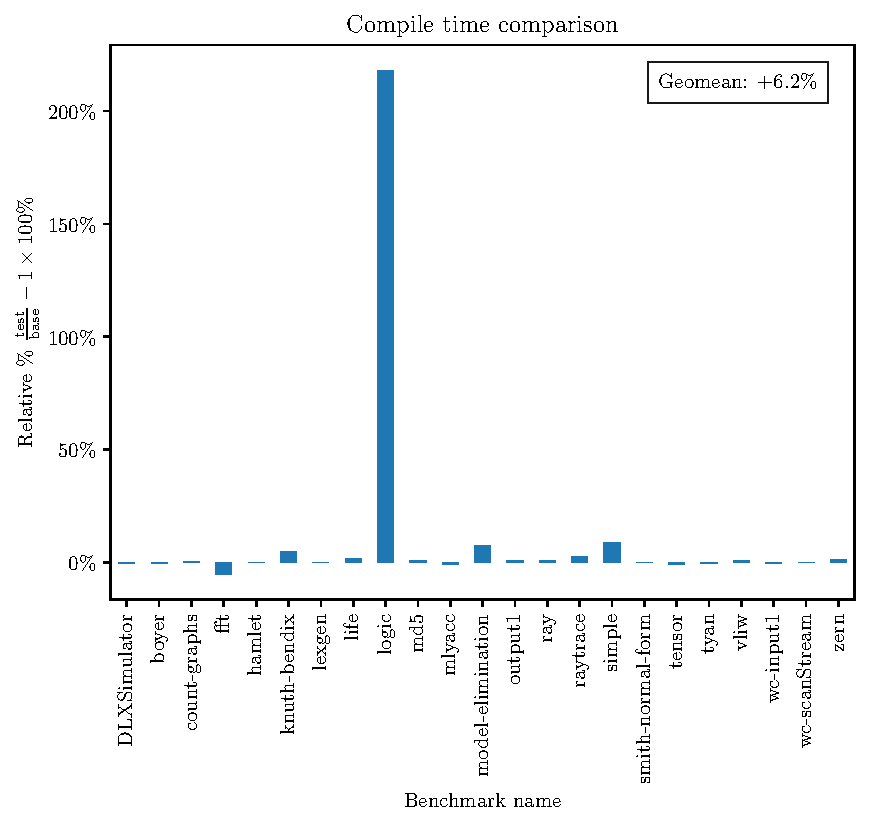
\includegraphics[width=\textwidth]{../analysis/charts/con_mlton_compile_mlton_vs_mlton.pdf}
    \caption{Compile time}
    \label{fig:con_mlton_compile_mlton_vs_mlton}
  \end{subfigure}
  \hfill
  \begin{subfigure}[b]{0.32\textwidth}
    \centering
    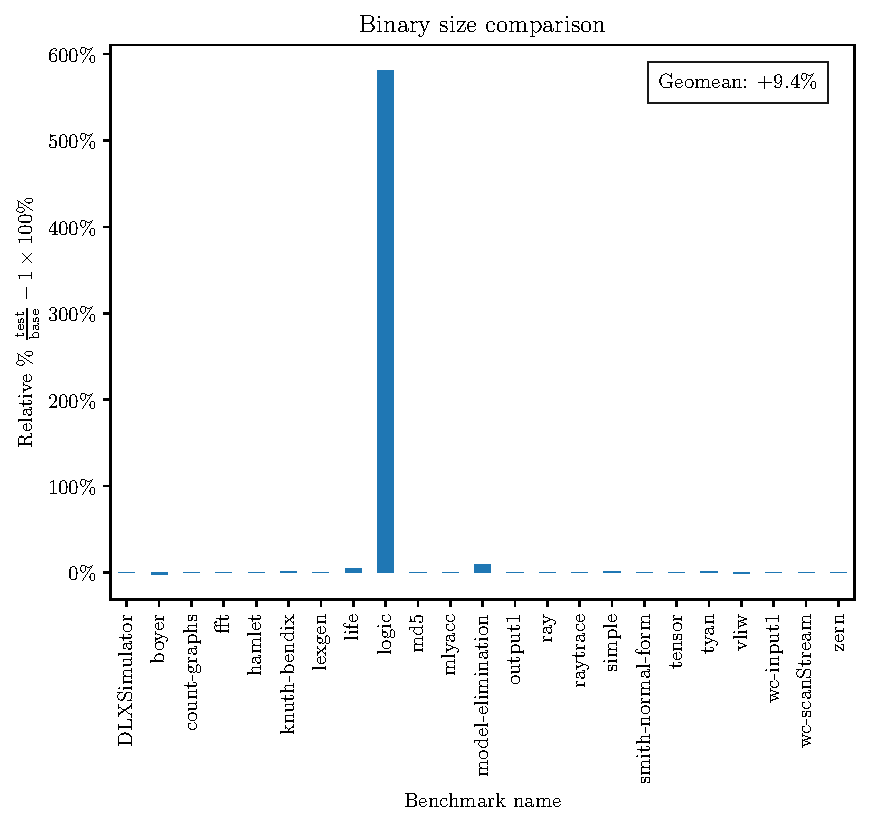
\includegraphics[width=\textwidth]{../analysis/charts/con_mlton_size_mlton_vs_mlton.pdf}
    \caption{Binary size}
    \label{fig:con_mlton_size_mlton_vs_mlton}
  \end{subfigure}
  \caption{Relative performance for with- vs without-\texttt{PreFlatten}, applied to \texttt{ConApp} on the MLton benchmark suite. <0\% represents an improvement, >0\% represents a regression.}
  \label{fig:con_mlton}
\end{figure}

\hl{TODO: THIS IS NOW A WIN}

The MLton benchmark suite shows modest $\approx 5\%$ regressions on a number of
benchmarks, for an overall geomean loss. We'll investiage the large loss to
\texttt{wc-input1} in the next section.

\subsection{\texttt{wc-input1}: detailed analysis}

The benchmark itself is simply a loop that reads from a buffered IO stream and
counts newlines:
\begin{minted}{sml}
fun loop (i: int): int =
  case input1 ins of
    NONE => i
  | SOME c => loop (if c = #"\n" then i + 1 else i)
\end{minted}
where \texttt{input1} is a standard library function that reads a single
character from a provided input stream (here, a temporary file).

The \texttt{ConApp} flattening pass makes the following changes:
\begin{itemize}
\item During initialization, it flattens the call to a string-concatenation routine
\item During runtime, it flattens calls to various functions that report errors
  in case of e.g. IO failure when reading the file.
\end{itemize}
No hot codepaths whatsoever are impacted. What is the cause of the regression?

Like above, we can run in \texttt{-chunkify one} in order to control for the
effect of chunkification, which is impacted by the introduction of any new
functons.

\hl{TODO: THE DATA CHANGED AND WE NEED TO REWORK THE ANALYSIS A BIT}

\FloatBarrier
\section{\texttt{wc-input1}: controlling for \texttt{Chunkify}}

As we can see in \cref{fig:mlton_bench_mlton_con_chunkify_one}, nearly the
entire positive effect of the transformation observed on the MLton benchmark
suite is actually due to accidental permutation of chunk boundaries rather than
the inded purpose of the pass -- the majr wins on \texttt{wc-input1} and
\texttt{wc-scanStream} disappear, and we are left with a small geomean loss
rather than a win.

\begin{figure}[htbp]
  \centering
  \includegraphics[width=\textwidth,keepaspectratio]{../analysis/charts/mlton_con_chunkify_one_mlton_bench.pdf}
  \caption{Comparison of benchmark performance for \texttt{ConApp} flattening on the MLton benchmark suite under MLton, comparing the baseline configuration against \texttt{-chunkify one}. <0\% represents an improvement, >0\% represents a regression.}
  \label{fig:mlton_bench_mlton_con_chunkify_one}
\end{figure}


\FloatBarrier
\section{\texttt{parallel-ml-bench}: MLton vs MLton}

\begin{figure}[htbp]
  \centering
  \begin{subfigure}[b]{0.48\textwidth}
    \centering
    \includegraphics[width=\textwidth]{../analysis/charts/con_parallel_bench_run_mlton_vs_mlton.pdf}
    \caption{Run time}
    \label{fig:con_parallel_bench_run_mlton_vs_mlton}
  \end{subfigure}
  \hfill
  \begin{subfigure}[b]{0.48\textwidth}
    \centering
    \includegraphics[width=\textwidth]{../analysis/charts/con_parallel_bench_size_mlton_vs_mlton.pdf}
    \caption{Binary size}
    \label{fig:con_parallel_bench_size_mlton_vs_mlton}
  \end{subfigure}
  \caption{Relative performance for with- vs without-\texttt{PreFlatten}, applied to \texttt{ConApp} on the \texttt{parallel-ml-bench} benchmark suite. <0\% represents an improvement, >0\% represents a regression.}
  \label{fig:con_parallel_bench}
\end{figure}

On \cref{fig:con_parallel_bench}, we see strong wins across a number of
benchmarks, and few losses, for a strong geomean win of $4.1\%$. To what degree
is this measurement impacted by chunkification noise, as we saw above?

The chart \cref{fig:con_parallel_bench_mlton_chunkify} plots the relative
performance of the default experimental setup alongside the relative performance
in a setup with \texttt{-chunkify one}. As we can see, the largest wins in
\texttt{linearrec} and \texttt{quickhull} persist: this suggests an
individually-meaningful impact of the \texttt{ConApp} flattening transformation,
unlike the \texttt{tuple} case.

However, it surfaces one significant loss on \texttt{mcss-opt} that likely
requires further investigation. We also see a number of significant wins
disappear (e.g. \texttt{primes} and \texttt{sparse-mxv-opt}), suggesting that
the baseline measurement does contain significant incidental performance changes
due to chunkification.

\begin{figure}[htbp]
  \centering
  \includegraphics[width=\textwidth,keepaspectratio]{../analysis/charts/mlton_con_chunkify_one_parallel_bench.pdf}
  \caption{Comparison of benchmark performance for \texttt{ConApp} flattening on \texttt{parallel-ml-bench} under MLton, comparing the baseline configuration against \texttt{-chunkify one}. <0\% represents an improvement, >0\% represents a regression.}
  \label{fig:con_parallel_bench_mlton_chunkify}
\end{figure}

\subsection{\texttt{parallel-ml-bench}: MPL vs MPL}

\begin{figure}[htbp]
  \centering
  \begin{subfigure}[b]{0.48\textwidth}
    \centering
    \includegraphics[width=\textwidth]{../analysis/charts/con_parallel_bench_run_mpl_vs_mpl_trellis.pdf}
    \caption{Run time}
    \label{fig:con_parallel_bench_run_mpl_vs_mpl}
  \end{subfigure}\hfill
  \begin{minipage}[b]{0.48\textwidth}
    \begin{subfigure}{\textwidth}
      \centering
      \includegraphics[width=\textwidth]{../analysis/charts/con_parallel_bench_run_mpl_vs_mpl_geomean.pdf}
      \caption{Geomean only}
      \label{fig:con_parallel_bench_geomean_mpl_vs_mpl}
    \end{subfigure}

    \begin{subfigure}{\textwidth}
      \centering
      \includegraphics[width=\textwidth]{../analysis/charts/con_parallel_bench_size_mpl_vs_mpl.pdf}
      \caption{Binary size}
      \label{fig:con_parallel_bench_size_mpl_vs_mpl}
    \end{subfigure}
  \end{minipage}
  \caption{Relative performance for with- vs without-\texttt{PreFlatten}, applied to \texttt{ConApp} on the \texttt{parallel-ml-bench} benchmark suite, for the MPL compiler, at a variety of core counts. <0\% represents an improvement, >0\% represents a regression.}
  \label{fig:con_parallel_bench_mpl}
\end{figure}

\hl{UPDATED THE CHARTS: NEED TO RE-CHECK THE BENCHMARK NAMES BELOW}

In the default experiment configuration, we see an overall loss for
\texttt{ConApp} flattening in MPL, driven primarily by a large, consistent
regression against \texttt{suffix-array}.

Re-running this particular benchmark under \texttt{-chunkify one} shows that the
effect disappears, as we can see in \cref{fig:con_chunkify_one_outliers}:
\texttt{suffix-array} is roughly neutral under \texttt{ConApp} flattening once
we control for chunkification. We can also see how the large swings reported by
\texttt{linearrec} change under \texttt{-chunkify one} in
\cref{fig:con_chunkify_one_outliers}: here, it appears that there is a
legitimate effect on the benchmark at higher core counts which merits further
investigation.

\begin{figure}[htbp]
  \centering
  \begin{subfigure}[b]{0.48\textwidth}
    \centering
    \includegraphics[width=\textwidth]{../analysis/charts/con_exp_suffix_array.pdf}
    \caption{\texttt{suffix-array}}
    \label{fig:con_exp_suffix_array}
  \end{subfigure}
  \hfill
  \begin{subfigure}[b]{0.48\textwidth}
    \centering
    \includegraphics[width=\textwidth]{../analysis/charts/con_exp_linearrec.pdf}
    \caption{\texttt{linearrec}}
    \label{fig:con_exp_linearrec}
  \end{subfigure}
  \caption{Comparison of speedups across core counts for \texttt{suffix-array} and \texttt{linearrec} under baseline \texttt{ConApp} flattening versus with \texttt{-chunkify one}. <0\% represents an improvement, >0\% represents a regression.}
  \label{fig:con_chunkify_one_outliers}
\end{figure}

In \cref{fig:con_chunkify_one_geomeans}, we see that (like \texttt{tuple}
flattening), the \texttt{ConApp} flattening transformation is broadly
neutral-to-positive when excluding chunk overhead. See
\cref{fig:mpl_con_chunkify_one_all} for the full set of experimental data for the
\texttt{-chunkify one} configuration.

\begin{figure}[htbp]
  \centering
  \includegraphics[width=\textwidth]{../analysis/charts/con_exp_geomean.pdf}
  \caption{Comparison of geometric mean speedups across core counts for baseline \texttt{ConApp} flattening versus with \texttt{-chunkify one}. <0\% represents an improvement, >0\% represents a regression.}
  \label{fig:con_chunkify_one_geomeans}
\end{figure}

\begin{figure}[htbp]
  \centering
  \includegraphics[width=\textwidth,height=0.88\textheight,keepaspectratio]{../analysis/charts/con_chunkify_one_parallel_bench_run_mpl_vs_mpl_trellis.pdf}
  \caption{Relative performance for \texttt{ConApp} flattening with \texttt{-chunkify one} on the \texttt{parallel-ml-bench} benchmark suite, for the MPL compiler, across core counts. <0\% represents an improvement, >0\% represents a regression.}
  \label{fig:mpl_con_chunkify_one_all}
  \label{mpl_con_chunkify_one_all}
\end{figure}

\FloatBarrier
\section{AoS Flattening}

\hl{TODO: CHECK -- 3 or 4 elements?}

In the data below, we applied the Array-of-Struct \texttt{ShallowFlatten}
transformation to all containers-of-tuples of less than or equal to 3 elements.

\subsection{MLton Benchmarks}

\begin{figure}[htbp]
  \centering
  \begin{subfigure}[b]{0.32\textwidth}
    \centering
    \includegraphics[width=\textwidth]{../analysis/charts/aos_mlton_run_mlton_vs_mlton.pdf}
    \caption{Run time}
    \label{fig:aos_mlton_run_mlton_vs_mlton}
  \end{subfigure}
  \hfill
  \begin{subfigure}[b]{0.32\textwidth}
    \centering
    \includegraphics[width=\textwidth]{../analysis/charts/aos_mlton_compile_mlton_vs_mlton.pdf}
    \caption{Compile time}
    \label{fig:aos_mlton_compile_mlton_vs_mlton}
  \end{subfigure}
  \hfill
  \begin{subfigure}[b]{0.32\textwidth}
    \centering
    \includegraphics[width=\textwidth]{../analysis/charts/aos_mlton_size_mlton_vs_mlton.pdf}
    \caption{Binary size}
    \label{fig:aos_mlton_size_mlton_vs_mlton}
  \end{subfigure}
  \caption{Relative performance for with- vs without-\texttt{ShallowFlatten}, using the AoS transformation on the MLton benchmark suite. <0\% represents an improvement, >0\% represents a regression.}
  \label{fig:aos_mlton}
\end{figure}

As we can see in \cref{fig:aos_mlton}, this transformation is essentially a
no-op on the MLton benchmark suite, impacting only a single benchmark for a win
smaller than 1\%.


\subsection{\texttt{parallel-ml-bench}: MLton vs MLton}

\begin{figure}[htbp]
  \centering
  \begin{subfigure}[b]{0.48\textwidth}
    \centering
    \includegraphics[width=\textwidth]{../analysis/charts/aos_parallel_bench_run_mlton_vs_mlton.pdf}
    \caption{Run time}
    \label{fig:aos_parallel_bench_run_mlton_vs_mlton}
  \end{subfigure}
  \hfill
  \begin{subfigure}[b]{0.48\textwidth}
    \centering
    \includegraphics[width=\textwidth]{../analysis/charts/aos_parallel_bench_size_mlton_vs_mlton.pdf}
    \caption{Binary size}
    \label{fig:aos_parallel_bench_size_mlton_vs_mlton}
  \end{subfigure}
  \caption{Relative performance for with- vs without-\texttt{ShallowFlatten}, using the AoS transformation on the \texttt{parallel-ml-bench} benchmark suite. <0\% represents an improvement, >0\% represents a regression.}
  \label{fig:aos_parallel_bench}
\end{figure}

AOS flattening has a largely poisitive impact on MLton for the
\texttt{parallel\_bench} suite. We'll focus on MPL for a more detailed analysis,
in the style of the previous sections.

\subsection{\texttt{parallel-ml-bench}: MPL vs MPL}

\begin{figure}[htbp]
  \centering
  \begin{subfigure}[b]{0.48\textwidth}
    \centering
    \includegraphics[width=\textwidth]{../analysis/charts/aos_parallel_bench_run_mpl_vs_mpl_trellis.pdf}
    \caption{Run time}
    \label{fig:aos_parallel_bench_run_mpl_vs_mpl}
  \end{subfigure}\hfill
  \begin{minipage}[b]{0.48\textwidth}
    \begin{subfigure}{\textwidth}
      \centering
      \includegraphics[width=\textwidth]{../analysis/charts/aos_parallel_bench_run_mpl_vs_mpl_geomean.pdf}
      \caption{Geomean only}
      \label{fig:aos_parallel_bench_geomean_mpl_vs_mpl}
    \end{subfigure}

    \begin{subfigure}{\textwidth}
      \centering
      \includegraphics[width=\textwidth]{../analysis/charts/aos_parallel_bench_size_mpl_vs_mpl.pdf}
      \caption{Binary size}
      \label{fig:aos_parallel_bench_size_mpl_vs_mpl}
    \end{subfigure}
  \end{minipage}
  \caption{Relative performance for with- vs without-\texttt{ShallowFlatten}, using the AoS transformation on the \texttt{parallel-ml-bench} benchmark suite, for the MPL compiler, at a variety of core counts. <0\% represents an improvement, >0\% represents a regression.}
  \label{fig:aos_parallel_bench_mpl}
\end{figure}

For MPL, the AOS transformation is overwhelmingly positive. For a deep dive,
we'll focus on two cases with large effects: \texttt{quickhull} (a large,
consistent win) and \texttt{linearrec} (a win at low core counts that becomes a
noisy loss at high core counts.

\subsection{\texttt{quickhull}, \texttt{linearrec}: observed IR change}
The \texttt{quickhull} benchmark calculates the convex hull of a 2D set of
points. In the particular implementation used in \texttt{parallel\_ml\_bench},
the core of the algorithm involves filtering a set of indices into two smaller
sets, e.g., very roughly:
\begin{minted}{python}
  points: (float * float) array = ...initialized on startup...
  def partition(indices: int list) -> (int array) * (int array):
    def is_left(index: int) -> bool:
      # Indexed load into `points`
      p: (float * float) = points[index]
      ...some 2D geometry calculation that loads points...

    def is_right(index: int) -> bool:
      ...similar...

    lefts: int list = filter(is_left, indices)
    right: int list = filter(is_right, indices)
    return (filter(is_left, indices), filter(is_right, indices))
  def quickhull(indices: int array, ...) -> int array:
    if len(indices) < C:
      ...base case...
    else:
      left, right = partition(indices)
      left_result = quickhull(left)
      right_result = quickhull(right)
      ...merge...
      return result
\end{minted}

The \texttt{linearrec} benchmark is quite simple, calculating a first-order
linear recurrence across a sequence of 2D points, i.e., in the scalar code:
\begin{minted}{python}
  points: (float * float) array = ...

  def linearrec(points):
    def combine(left: (float * float), right: (float * float)) -> (float * float):
      l_x, l_y = left
      r_x, r_y = right
      return (l_x * r_x, l_y * r_x + r_y)

    def select(point: float * float) -> float:
      l, r = point
      return l

    identity = (1.0, 0.0)
    # Prefix scan over pairs with `combine`
    points' = list(prefix_scan(pairs, combine))
    return [select(p) for p in points']
\end{minted}
where \texttt{prefix\_scan} is an MPL primitive that calculates the parallel
prefix scan of the associative \texttt{combine} operator, i.e. the sequence:
\begin{minted}{python}
  identity = (1.0, 0.0)
  points' = [combine(identity, points[0]),
             combine(points'[0], points[1]),
             combine(points'[1], points[2]),
             ...]
\end{minted}
through a standard paralell prefix scan algorithm that completes the task in
$O(n)$ total work and a critical path length of $O(\log n)$ operations.

The transformations here are straightforward: for \texttt{quickhull}, we rewrite
the global \texttt{points} array into array-of-structs format:
\begin{minted}{python}
  points: float array = ...initialized on startup...
  def partition(indices: int list) -> (int array) * (int array):
    def is_left(index: int) -> bool:
      # Indexed load into `points`
      p_x: float = points[index * 2]
      p_y: float = points[index * 2 + 1]
      # Temporary tuple produced by the `ShallowFlatten` transformation
      p: float * float = (p_x, p_y)
      ...some 2D geometry calculation that loads points...

    def is_right(index: int) -> bool:
      ...similar...

  ...as above...
\end{minted}
where the temporary tuple \texttt{p} is successfully eliminated by later passes,
allowing the 2D geometry calculation operate directly on the unboxed values.

The transformation on \texttt{linearrec} is similarly obvious -- however, the IR
snippet from above remains unchaned because the transformation changes the body
of \texttt{parallel\_scan} to calculate a prefix sum over a flat \texttt{float *
  float} array. Later passes ensure that all temporary tuples are optimized
away, such that \texttt{ShallowFlatten} introduces no new allocations.

One important difference to note between \texttt{linearrec} and
\texttt{quickhull} is that, while \texttt{quickhull} only allocates
arrays-of-tuples at startup, \texttt{linearrec} allocates arrays of tuples at
runtime as well -- temporary arrays while computing the prefix scan. Thus for
\texttt{quickhull}, we observe only the effect of the transformation on the
generated code, but in \texttt{linearrec} we can also observe the interaction
with the garbage collector.



\subsection{\texttt{quickhull}, \texttt{linearrec}: microarchitectural effects}
Next, we walk through the same \texttt{perf}-centered analysis to determine how
the AOS transformation impacted the workload at a microarchitectural level. In
both cases, the effect we expect to see is the one described in the sections
above \hl{TODO LINK TO THE MEAT SECTION} -- in the cases where loading from the
2D point arrays is important for performance, saving the intermediate tuple
should save both memory latency (i.e. an extra dependent load operation --
shortening the chain length from 3 to 2 for \texttt{quickhull} and from 2 to 1
for \texttt{linearrec}) and memory bandwidth (we should be able to use the whole
cacheline that each point is allocated on).

For \texttt{quickhull}, we can see the single-threaded effect in
\cref{tab:perf_comparison_aos_quickhull_1core}. We observe, broadly, the effect
that we expect: we see better locality show up as a lower miss rate in both L1
and L3, translating into higher IPC. In additon to higher IPC, we also see a
reduction in total instructions, matching out expectations (since the packed AOS
loads require fewer instructions than the unpacked tuple loads, so long as the
intermediate tuples are optimized away). \hl{TODO: WHY BAD SPEC? LOWER MISS RATE
  SHOUHD SHOW UP AS LESS BACKEND BOUND}

Comparing with the 160 core data in
\cref{tab:perf_comparison_aos_quickhull_160cores}, trend for \texttt{quickhull}
is similar to the benchmarks we analyzed above, with the microarchitectural
bottleneck shifting from bad speculation towards backend bound as contention on
the memory subsystem increases.

For \texttt{linearrec}, the primary effect we observe in the single core data
from \cref{tab:perf_comparison_aos_linearrec_1core} is a massive reduction in
instruction count, which again corresponds with what we expect based on the
action of the transformation. Here, we see a slightly higher L1 miss rate
alongside a lower L3 miss rate, which we could explain as follows: for the
baseline verison, we tend to keep the pointers-to-tuples in L1 (i.e. the array
of pointers is small and has good locality) and miss in L3 when we load through
the poiners, whereas in the AOS version, the packed array is large enough to
exceed the size of L1, but we still have enough locality to keep it in lower
levels of the cache hierachy.



\hl{TODO: EXPLAIN THE INSTRUCTIONS / IPC / BADSPEC FOR LINEARREC AS GC}

\hl{TODO: DIG INTO THIS FURTHER USING PERF RECORD TO COLLECT THE ACTUAL DATA}

\hl{TODO: WRITEUP}

  1. Quickhull on 1 Core

    \begin{table}[htbp]
      \centering
      \caption{AoS performance metric comparison on 1 core (Quickhull, 1 core)}
      \label{tab:perf_comparison_aos_quickhull_1core}
      \begin{tabular}{lrrr}
        \toprule
        \textbf{Metric} & \textbf{Baseline} & \textbf{Test} & \textbf{Diff / Change} \\
        \midrule
        \multicolumn{4}{l}{\textit{Execution Overview}} \\
        \quad Task Clock (s)           & 49.53 s   & 36.65 s   & -26.00\%   \\
        \quad Instructions ($10^9$)    & 233.33 B  & 175.11 B  & -24.95\%   \\
        \quad IPC                      & 1.59       & 1.61       & +1.26\%    \\
        \midrule
        \multicolumn{4}{l}{\textit{Rates and Miss Percentages}} \\
        \quad Branch Miss Rate         & 1.7\%      & 2.2\%      & +0.5 pp    \\
        \quad L1 D-Cache Miss Rate     & 3.5\%      & 2.2\%      & -1.3 pp    \\
        \quad LLC Load Miss Rate       & 63.5\%     & 48.4\%     & -15.1 pp   \\
        \quad dTLB Load Miss Rate      & 0.1\%      & 0.1\%      & 0.0 pp     \\
        \midrule
        \multicolumn{4}{l}{\textit{Topdown L1 Metrics}} \\
        \quad Retiring                 & 2.6\%      & 5.3\%      & +2.7 pp    \\
        \quad Bad Speculation          & 88.9\%     & 85.6\%     & -3.3 pp    \\
        \quad Frontend Bound           & 0.3\%      & 0.3\%      & 0.0 pp     \\
        \quad Backend Bound            & 8.3\%      & 8.8\%      & +0.5 pp    \\
        \bottomrule
      \end{tabular}
    \end{table}

  2. Quickhull on 160 Cores

    \begin{table}[htbp]
      \centering
      \caption{AoS performance metric comparison on 160 cores (Quickhull, 160 cores)}
      \label{tab:perf_comparison_aos_quickhull_160cores}
      \begin{tabular}{lrrr}
        \toprule
        \textbf{Metric} & \textbf{Baseline} & \textbf{Test} & \textbf{Diff / Change} \\
        \midrule
        \multicolumn{4}{l}{\textit{Execution Overview}} \\
        \quad Task Clock (s)           & 213.50 s   & 120.36 s   & -43.63\%   \\
        \quad Instructions ($10^9$)    & 304.11 B  & 238.45 B  & -21.59\%   \\
        \quad IPC                      & 0.50       & 0.70       & +40.00\%   \\
        \midrule
        \multicolumn{4}{l}{\textit{Rates and Miss Percentages}} \\
        \quad Branch Miss Rate         & 1.4\%      & 1.7\%      & +0.3 pp    \\
        \quad L1 D-Cache Miss Rate     & 4.7\%      & 3.2\%      & -1.5 pp    \\
        \quad LLC Load Miss Rate       & 68.7\%     & 60.2\%     & -8.5 pp    \\
        \quad dTLB Load Miss Rate      & 0.1\%      & 0.1\%      & 0.0 pp     \\
        \midrule
        \multicolumn{4}{l}{\textit{Topdown L1 Metrics}} \\
        \quad Retiring                 & 3.8\%      & 9.6\%      & +5.8 pp    \\
        \quad Bad Speculation          & 64.6\%     & 59.3\%     & -5.3 pp    \\
        \quad Frontend Bound           & 0.9\%      & 1.9\%      & +1.0 pp    \\
        \quad Backend Bound            & 30.7\%      & 29.2\%      & -1.5 pp    \\
        \bottomrule
      \end{tabular}
    \end{table}

  3. Linearrec on 1 Core

    \begin{table}[htbp]
      \centering
      \caption{AoS performance metric comparison on 1 core (Linearrec, 1 core)}
      \label{tab:perf_comparison_aos_linearrec_1core}
      \begin{tabular}{lrrr}
        \toprule
        \textbf{Metric} & \textbf{Baseline} & \textbf{Test} & \textbf{Diff / Change} \\
        \midrule
        \multicolumn{4}{l}{\textit{Execution Overview}} \\
        \quad Task Clock (s)           & 86.98 s   & 43.11 s   & -50.44\%   \\
        \quad Instructions ($10^9$)    & 827.40 B  & 224.58 B  & -72.86\%   \\
        \quad IPC                      & 3.20       & 1.75       & -45.31\%   \\
        \midrule
        \multicolumn{4}{l}{\textit{Rates and Miss Percentages}} \\
        \quad Branch Miss Rate         & 0.0\%      & 0.0\%      & 0.0 pp     \\
        \quad L1 D-Cache Miss Rate     & 1.5\%      & 2.6\%      & +1.1 pp    \\
        \quad LLC Load Miss Rate       & 24.7\%     & 20.5\%     & -4.2 pp    \\
        \quad dTLB Load Miss Rate      & 0.0\%      & 0.0\%      & 0.0 pp     \\
        \midrule
        \multicolumn{4}{l}{\textit{Topdown L1 Metrics}} \\
        \quad Retiring                 & 3.3\%      & 8.0\%      & +4.7 pp    \\
        \quad Bad Speculation          & 94.6\%     & 81.5\%     & -13.1 pp   \\
        \quad Frontend Bound           & 0.1\%      & 0.9\%      & +0.8 pp    \\
        \quad Backend Bound            & 2.0\%      & 9.7\%      & +7.7 pp    \\
        \bottomrule
      \end{tabular}
    \end{table}

  4. Linearrec on 160 Cores

    \begin{table}[htbp]
      \centering
      \caption{AoS performance metric comparison on 160 cores (Linearrec, 160 cores)}
      \label{tab:perf_comparison_aos_linearrec_160cores}
      \begin{tabular}{lrrr}
        \toprule
        \textbf{Metric} & \textbf{Baseline} & \textbf{Test} & \textbf{Diff / Change} \\
        \midrule
        \multicolumn{4}{l}{\textit{Execution Overview}} \\
        \quad Task Clock (s)           & 391.07 s   & 555.27 s   & +41.99\%   \\
        \quad Instructions ($10^9$)    & 902.57 B  & 1321.08 B  & +46.37\%   \\
        \quad IPC                      & 0.80       & 0.82       & +2.50\%    \\
        \midrule
        \multicolumn{4}{l}{\textit{Rates and Miss Percentages}} \\
        \quad Branch Miss Rate         & 0.1\%      & 0.0\%      & -0.1 pp    \\
        \quad L1 D-Cache Miss Rate     & 5.3\%      & 5.9\%      & +0.6 pp    \\
        \quad LLC Load Miss Rate       & 26.1\%     & 20.5\%     & -5.6 pp    \\
        \quad dTLB Load Miss Rate      & 0.0\%      & 0.0\%      & 0.0 pp     \\
        \midrule
        \multicolumn{4}{l}{\textit{Topdown L1 Metrics}} \\
        \quad Retiring                 & 8.7\%      & 7.5\%      & -1.2 pp    \\
        \quad Bad Speculation          & 61.1\%     & 71.6\%     & +10.5 pp   \\
        \quad Frontend Bound           & 3.4\%      & 2.0\%      & -1.4 pp    \\
        \quad Backend Bound            & 26.9\%      & 18.9\%      & -8.0 pp    \\
        \bottomrule
      \end{tabular}
    \end{table}

\subsection{\texttt{quickhull}, \texttt{linearrec}: control for known effects}
Looking at per-trial data in \cref{fig:quickhull_linearrec_aos_scatter_plot}, we
see a clear difference between the two benchmarks: while \texttt{quickhull} has
fairly stable performance from trial to trial at all core counts,
\texttt{linearrec} shows a clear bimodal pattern, alternating between fast and
slow iterations on both sides.

It seems likely that this is an effect from the garbage collector: as described
in \citet{mpl-orig}, running hte MPL garbage collector has the effect of pausing
one of the worker threads, and hence for workloads with a uniform balance of
work between worker threads (like \texttt{linearrec}, whose innermost loop is
identical across processors), we should expect the GC pause to land on the
critical path. Since all units of work take nearly the same time, there is no
option to hide latency.

For the \texttt{linearrec} case, we can make an argument that changing
allocation patterns introduces ``noise'' by permuting the location of GC pauses:
executing the prefix scan algorithm involves a fanout of tasks, where each node
consumes some roughly-fixed time. For any given node, there is some probability
that a GC pause ``lands'' on that node, and the higher up in the tree the GC
pause lands, the more parallelism is wasted (since the GC pause blocks child
tasks at lower levels in the tree from spawing). \hl{TODO: need a diagram here}

Noting from \cref{fig:quickhull_linearrec_aos_scatter_plot} note that the
benchmarks run for a fixed time, the faster AOS-transformed version runes for
many more trials than the baseline. If there is a fixed chance that any
particular trial encounters an unlucky GC pause, then we should expect to see
both a larger number of unlucky trials and more-unlucky GC pauses on the side
whose non-unlucky runs are faster.

Thus we can attempt to isolate the effect of the GC in two ways:
\begin{enumerate}
\item We can run the benchmarks for a fixed trial count rather than a fixed
  duration: this tries to control for only the unlucky-trials effect, but
  retains some ``noise,'' since the AOS side will still have different
  allocation patterns and so generally tend to pause in a slightly different
  location.

\item We can eliminate the effect of GC pause placement entirely by running a
  synchronous GC at the beginning of each trial iteration. This, unfortunately,
  ``controls for too much'' by entirely removing the MPL GC heuristics from the
  benchmark, but still provides useful signal.
\end{enumerate}

Starting from the first point,
\cref{fig:quickhull_linearrec_aos_fixed_trials} compares our default
configuration against a configuration where all benchmarks run for a fixed trial
count. As we observe, the fixed trial conunt consistently reports larger wins
than the fixed time, but still shows noisy losses for \texttt{linearrec} at high
core counts. This experiment was run by changing the benchmark framework to use
a fixed iteration count for both trials and warmup, and selecting the trial
count based on the previously-observed completed runs in the non-AOS plain MPL
configuration -- the number of trials is consequently smaller than in the
default experiment configuration, and hence the error bars are larger. The shape
of this data is broadly the same as our baseline configuration; see
\cref{fig:aos_full_fixed_trial} for the complete dataset.

For the second point, we arrange for a synchronous GC by:
\begin{enumerate}
\item Passing \texttt{max-cc-depth 0 min-collection-depth 1} to the MPL runtime
  on both sides
\item Adding a call to \texttt{MLton.GC.Collect} at the start of each benchmark iteration
\end{enumerate}

The \texttt{MLton.GC.Collect} call is included in the timed region, and hence
the effect is simply to control the placement of GC pauses, not to remove the GC
effect entirely.

See \cref{fig:quickhull_linearrec_aos_sync_gc} for the results on our focus
benchmarks: as we see, the effect of worse relative performance at high core
counts is completley eliminated; both \texttt{quickhull} and \texttt{linearrec}
show performance improvements that increase monotonically with core count. This
effect holds for the other benchmarks in the suite: see
\cref{fig:aos_full_sync_gc} for the complete dataset.

Finally, as a quick test of methodology, we examine the effect of the
\texttt{-chunkify one} transformation on the AOS benchmark: given that the
transformation does not impact function boundaries, we should expect to see no
effect here, and this data point would help to confirm that ``controlling for
function boundary effects'' in the previous experiments did not have other,
unintended effects.

See \cref{fig:quickhull_linearrec_aos_chunkify_one} for the results on the focus
benchmarks. As expected, the effect is broadly neutral. See
\cref{fig:aos_full_chunkify_one} for the complete results in this configuration.


\begin{figure}[htbp]
  \centering
  \begin{subfigure}[b]{0.48\textwidth}
    \centering
    \includegraphics[width=\textwidth]{../analysis/charts/quickhull_default_aos_mpl_parallel_ml_bench_scatter.pdf}
    \caption{\texttt{quickhull}}
    \label{fig:quickhull_default_aos_mpl_parallel_ml_bench_scatter}
  \end{subfigure}
  \hfill
  \begin{subfigure}[b]{0.48\textwidth}
    \centering
    \includegraphics[width=\textwidth]{../analysis/charts/linearrec_default_aos_mpl_parallel_ml_bench_scatter.pdf}
    \caption{\texttt{linearrec}}
    \label{fig:linearrec_default_aos_mpl_parallel_ml_bench_scatter}
  \end{subfigure}
  \caption{Trial-by-trial execution time for \texttt{quickhull} and \texttt{linearrec} across core counts under default AoS flattening versus baseline for the MPL compiler.}
  \label{fig:quickhull_linearrec_aos_scatter_plot}
\end{figure}

\begin{figure}[htbp]
  \centering
  \begin{subfigure}[b]{0.32\textwidth}
    \centering
    \includegraphics[width=\textwidth]{../analysis/charts/aos_fixed_iters_geomean.pdf}
    \caption{Geometric mean}
    \label{fig:aos_fixed_iters_geomean}
  \end{subfigure}
  \hfill
  \begin{subfigure}[b]{0.32\textwidth}
    \centering
    \includegraphics[width=\textwidth]{../analysis/charts/aos_fixed_iters_quickhull.pdf}
    \caption{\texttt{quickhull}}
    \label{fig:aos_fixed_iters_quickhull}
  \end{subfigure}
  \hfill
  \begin{subfigure}[b]{0.32\textwidth}
    \centering
    \includegraphics[width=\textwidth]{../analysis/charts/aos_fixed_iters_linearrec.pdf}
    \caption{\texttt{linearrec}}
    \label{fig:aos_fixed_iters_linearrec}
  \end{subfigure}
  \caption{Comparison of speedups across core counts for geometric mean, \texttt{quickhull}, and \texttt{linearrec} under default AoS flattening versus fixed iteration count (fixed trials). <0\% represents an improvement, >0\% represents a regression.}
  \label{fig:quickhull_linearrec_aos_fixed_trials}
  \label{fig_quickhull_linearrec_aos_fixed_trials}
\end{figure}

\begin{figure}[htbp]
  \centering
  \includegraphics[width=\textwidth,height=0.88\textheight,keepaspectratio]{../analysis/charts/aos_fixed_iters_parallel_bench_run_mpl_vs_mpl_trellis.pdf}
  \caption{Relative performance for AoS flattening with fixed trial counts on the \texttt{parallel-ml-bench} benchmark suite, for the MPL compiler, across core counts. <0\% represents an improvement, >0\% represents a regression.}
  \label{fig:aos_full_fixed_trial}
\end{figure}

\begin{figure}[htbp]
  \centering
  \begin{subfigure}[b]{0.32\textwidth}
    \centering
    \includegraphics[width=\textwidth]{../analysis/charts/aos_sync_gc_geomean.pdf}
    \caption{Geometric mean}
    \label{fig:aos_sync_gc_geomean}
  \end{subfigure}
  \hfill
  \begin{subfigure}[b]{0.32\textwidth}
    \centering
    \includegraphics[width=\textwidth]{../analysis/charts/aos_sync_gc_quickhull.pdf}
    \caption{\texttt{quickhull}}
    \label{fig:aos_sync_gc_quickhull}
  \end{subfigure}
  \hfill
  \begin{subfigure}[b]{0.32\textwidth}
    \centering
    \includegraphics[width=\textwidth]{../analysis/charts/aos_sync_gc_linearrec.pdf}
    \caption{\texttt{linearrec}}
    \label{fig:aos_sync_gc_linearrec}
  \end{subfigure}
  \caption{Comparison of speedups across core counts for geometric mean, \texttt{quickhull}, and \texttt{linearrec} under default AoS flattening versus synchronous GC. <0\% represents an improvement, >0\% represents a regression.}
  \label{fig:quickhull_linearrec_aos_sync_gc}
\end{figure}

\begin{figure}[htbp]
  \centering
  \includegraphics[width=\textwidth,height=0.88\textheight,keepaspectratio]{../analysis/charts/aos_sync_gc_parallel_bench_run_mpl_vs_mpl_trellis.pdf}
  \caption{Relative performance for AoS flattening with synchronous GC on the \texttt{parallel-ml-bench} benchmark suite, for the MPL compiler, across core counts. <0\% represents an improvement, >0\% represents a regression.}
  \label{fig:aos_full_sync_gc}
\end{figure}

\begin{figure}[htbp]
  \centering
  \begin{subfigure}[b]{0.32\textwidth}
    \centering
    \includegraphics[width=\textwidth]{../analysis/charts/aos_chunkify_one_geomean.pdf}
    \caption{Geometric mean}
    \label{fig:aos_chunkify_one_geomean}
  \end{subfigure}
  \hfill
  \begin{subfigure}[b]{0.32\textwidth}
    \centering
    \includegraphics[width=\textwidth]{../analysis/charts/aos_chunkify_one_quickhull.pdf}
    \caption{\texttt{quickhull}}
    \label{fig:aos_chunkify_one_quickhull}
  \end{subfigure}
  \hfill
  \begin{subfigure}[b]{0.32\textwidth}
    \centering
    \includegraphics[width=\textwidth]{../analysis/charts/aos_chunkify_one_linearrec.pdf}
    \caption{\texttt{linearrec}}
    \label{fig:aos_chunkify_one_linearrec}
  \end{subfigure}
  \caption{Comparison of speedups across core counts for geometric mean, \texttt{quickhull}, and \texttt{linearrec} under default AoS flattening versus AoS with \texttt{-chunkify one}. <0\% represents an improvement, >0\% represents a regression.}
  \label{fig:quickhull_linearrec_aos_chunkify_one}
\end{figure}

\begin{figure}[htbp]
  \centering
  \includegraphics[width=\textwidth,height=0.88\textheight,keepaspectratio]{../analysis/charts/aos_chunkify_one_parallel_bench_run_mpl_vs_mpl_trellis.pdf}
  \caption{Relative performance for AoS flattening with \texttt{-chunkify one} on the \texttt{parallel-ml-bench} benchmark suite, for the MPL compiler, across core counts. <0\% represents an improvement, >0\% represents a regression.}
  \label{fig:aos_full_chunkify_one}
\end{figure}

\FloatBarrier
\section{SoA Flattening}

\hl{TODO: CHECK -- 3 or 4 elements?}

In the data below, we applied the Struct-of-Array \texttt{ShallowFlatten}
transformation to all containers-of-tuples of less than or equal to 3 elements.

\subsection{MLton Benchmarks}

\begin{figure}[htbp]
  \centering
  \begin{subfigure}[b]{0.32\textwidth}
    \centering
    \includegraphics[width=\textwidth]{../analysis/charts/soa_mlton_run_mlton_vs_mlton.pdf}
    \caption{Run time}
    \label{fig:soa_mlton_run_mlton_vs_mlton}
  \end{subfigure}
  \hfill
  \begin{subfigure}[b]{0.32\textwidth}
    \centering
    \includegraphics[width=\textwidth]{../analysis/charts/soa_mlton_compile_mlton_vs_mlton.pdf}
    \caption{Compile time}
    \label{fig:soa_mlton_compile_mlton_vs_mlton}
  \end{subfigure}
  \hfill
  \begin{subfigure}[b]{0.32\textwidth}
    \centering
    \includegraphics[width=\textwidth]{../analysis/charts/soa_mlton_size_mlton_vs_mlton.pdf}
    \caption{Binary size}
    \label{fig:soa_mlton_size_mlton_vs_mlton}
  \end{subfigure}
  \caption{Relative performance for with- vs without-\texttt{ShallowFlatten}, using the SoA transformation on the MLton benchmark suite. <0\% represents an improvement, >0\% represents a regression.}
  \label{fig:soa_mlton}
\end{figure}

The effect here, like in \cref{fig:aos_mlton}, is essentially negligible.

\subsection{\texttt{parallel-ml-bench}: MLton vs MLton}

\begin{figure}[htbp]
  \centering
  \begin{subfigure}[b]{0.48\textwidth}
    \centering
    \includegraphics[width=\textwidth]{../analysis/charts/soa_parallel_bench_run_mlton_vs_mlton.pdf}
    \caption{Run time}
    \label{fig:soa_parallel_bench_run_mlton_vs_mlton}
  \end{subfigure}
  \hfill
  \begin{subfigure}[b]{0.48\textwidth}
    \centering
    \includegraphics[width=\textwidth]{../analysis/charts/soa_parallel_bench_size_mlton_vs_mlton.pdf}
    \caption{Binary size}
    \label{fig:soa_parallel_bench_size_mlton_vs_mlton}
  \end{subfigure}
  \caption{Relative performance for with- vs without-\texttt{ShallowFlatten}, using the SoA transformation on the \texttt{parallel-ml-bench} benchmark suite. <0\% represents an improvement, >0\% represents a regression.}
  \label{fig:soa_parallel_bench}
  \label{fig:soa_mlton_bench}
\end{figure}

See \cref{fig:soa_mlton_bench} for the impact of the SoA transformation on the
\texttt{parallel\_bench} suite for the MLton compiler.

While the geomean impact of the transformation is broadly the same between AoS
and SoA, we can see directionally-different results in some cases -- most
significantly, \texttt{delaunay} is a small win for the AoS configuration, but a
significant loss for the SoA configuration. See
\cref{fig:mlton_aos_vs_soa_parallel_bench} for a side-by-side comparison.

\begin{figure}[htbp]
  \centering
  \includegraphics[width=\textwidth,keepaspectratio]{../analysis/charts/mlton_aos_vs_soa_parallel_bench.pdf}
  \caption{Comparison of benchmark performance for AoS versus SoA flattening on the \texttt{parallel-ml-bench} benchmark suite under MLton. <0\% represents an improvement, >0\% represents a regression.}
  \label{fig:mlton_aos_vs_soa_parallel_bench}
\end{figure}

To diagnose the slowdown, we can briefly dig into microarchitectural data again.

For a win that is consistent across both AoS and SoA, we can inspect
\cref{tab:perf_comparison_soa_linearrec_1core} and
\cref{tab:perf_comparison_aos_linearrec_1core}. Both AoS and SoA exhbit improved
IPC and reduced DRAM traffic, with AoS at a higher instruction count but a lower
IPC, and SoA at a lower instruction count at a higher IPC. The metrics suggest
that in the SoA flavor, we have better locality for the array operations
themselves, but some extra tuple pack/unpack operations, whereas in the AoS
flavor, the workload pushes some hot data out of L1, but we do fewer tuple
pack/unpack operations.

By contrast, comparing \cref{tab:perf_comparison_soa_delaunay_1core} with
\cref{tab:perf_comparison_aos_delaunay_1core}, we see a sharp drop in IPC for
the SoA version as compared to the AoS version, at roughly a fixed instruction
count. Here, the measures of cache locality show a sharp decrease in the SoA
version -- the increase in dTLB miss rate suggests that the SoA layout results
in the algorith thrashing across extremely distant memory addreses.

One possible explanation is the following: for the SoA layout, unlike the AoS
layout, we do separate allocations for each of the members of the
struct-of-arrays. If the data in the struct is large, we need to request a new
page from the host OS for each allocation, and so struct members end up
scattered across unrelated pages. Additionally, we need to suppose that the
inner loop of the algorithm touches a large-enough chunk of memory such that one
of the scattered struct members ends up pushed to a lower level of the cache
hierarchy (indicated by the increase in L1 misses) or pushed out entirely
(indicated by the indcrease in LLC misses).

\hl{TODO: how does the memory allocator work?}

    \begin{table}[htbp]
      \centering
      \caption{AoS performance metric comparison on 1 core (Delaunay, 1 core)}
      \label{tab:perf_comparison_aos_delaunay_1core}
      \begin{tabular}{lrrr}
        \toprule
        \textbf{Metric} & \textbf{Baseline} & \textbf{Test} & \textbf{Diff / Change} \\
        \midrule
        \multicolumn{4}{l}{\textit{Execution Overview}} \\
        \quad Task Clock (s)           & 97.69 s   & 96.22 s   & -1.50\%   \\
        \quad Instructions ($10^9$)    & 248.33 B  & 250.89 B  & +1.03\%   \\
        \quad IPC                      & 0.86       & 0.88       & +2.33\%    \\
        \midrule
        \multicolumn{4}{l}{\textit{Rates and Miss Percentages}} \\
        \quad Branch Miss Rate         & 3.8\%      & 3.9\%      & +0.1 pp     \\
        \quad L1 D-Cache Miss Rate     & 11.9\%      & 12.0\%      & +0.1 pp    \\
        \quad LLC Load Miss Rate       & 17.6\%     & 16.9\%     & -0.7 pp    \\
        \quad dTLB Load Miss Rate      & 2.5\%      & 2.6\%      & +0.1 pp     \\
        \midrule
        \multicolumn{4}{l}{\textit{Topdown L1 Metrics}} \\
        \quad Retiring                 & 1.9\%      & 1.9\%      & 0.0 pp    \\
        \quad Bad Speculation          & 83.6\%     & 83.5\%     & -0.1 pp   \\
        \quad Frontend Bound           & 0.0\%      & 0.0\%      & 0.0 pp    \\
        \quad Backend Bound            & 14.5\%      & 14.6\%      & +0.1 pp    \\
        \bottomrule
      \end{tabular}
    \end{table}

        \begin{table}[htbp]
      \centering
      \caption{SoA performance metric comparison on 1 core (Delaunay, 1 core)}
      \label{tab:perf_comparison_soa_delaunay_1core}
      \begin{tabular}{lrrr}
        \toprule
        \textbf{Metric} & \textbf{Baseline} & \textbf{Test} & \textbf{Diff / Change} \\
        \midrule
        \multicolumn{4}{l}{\textit{Execution Overview}} \\
        \quad Task Clock (s)           & 97.84 s   & 120.30 s   & +22.96\%   \\
        \quad Instructions ($10^9$)    & 246.62 B  & 246.92 B  & +0.12\%   \\
        \quad IPC                      & 0.85       & 0.69       & -18.82\%    \\
        \midrule
        \multicolumn{4}{l}{\textit{Rates and Miss Percentages}} \\
        \quad Branch Miss Rate         & 3.8\%      & 4.1\%      & +0.3 pp     \\
        \quad L1 D-Cache Miss Rate     & 11.9\%      & 17.0\%      & +5.1 pp    \\
        \quad LLC Load Miss Rate       & 16.9\%     & 17.4\%     & +0.5 pp    \\
        \quad dTLB Load Miss Rate      & 2.5\%      & 5.4\%      & +2.9 pp     \\
        \midrule
        \multicolumn{4}{l}{\textit{Topdown L1 Metrics}} \\
        \quad Retiring                 & 1.9\%      & 1.7\%      & -0.2 pp    \\
        \quad Bad Speculation          & 83.8\%     & 82.1\%     & -1.7 pp   \\
        \quad Frontend Bound           & 0.0\%      & 0.1\%      & +0.1 pp    \\
        \quad Backend Bound            & 14.5\%      & 16.1\%      & +1.6 pp    \\
        \bottomrule
      \end{tabular}
    \end{table}

        \begin{table}[htbp]
      \centering
      \caption{AoS performance metric comparison on 1 core (Linearrec, 1 core)}
      \label{tab:perf_comparison_aos_linearrec_1core}
      \begin{tabular}{lrrr}
        \toprule
        \textbf{Metric} & \textbf{Baseline} & \textbf{Test} & \textbf{Diff / Change} \\
        \midrule
        \multicolumn{4}{l}{\textit{Execution Overview}} \\
        \quad Task Clock (s)           & 57.80 s   & 26.45 s   & -54.24\%   \\
        \quad Instructions ($10^9$)    & 304.44 B  & 150.59 B  & -50.54\%   \\
        \quad IPC                      & 1.77       & 1.92       & +8.47\%    \\
        \midrule
        \multicolumn{4}{l}{\textit{Rates and Miss Percentages}} \\
        \quad Branch Miss Rate         & 0.0\%      & 0.0\%      & 0.0 pp     \\
        \quad L1 D-Cache Miss Rate     & 5.2\%      & 6.5\%      & +1.3 pp    \\
        \quad LLC Load Miss Rate       & 47.6\%     & 37.2\%     & -10.4 pp    \\
        \quad dTLB Load Miss Rate      & 0.0\%      & 0.0\%      & 0.0 pp     \\
        \midrule
        \multicolumn{4}{l}{\textit{Topdown L1 Metrics}} \\
        \quad Retiring                 & 6.3\%      & 11.0\%      & +4.7 pp    \\
        \quad Bad Speculation          & 82.4\%     & 73.9\%     & -8.5 pp   \\
        \quad Frontend Bound           & 1.9\%      & 3.6\%      & +1.7 pp    \\
        \quad Backend Bound            & 9.4\%      & 11.5\%      & +2.1 pp    \\
        \bottomrule
      \end{tabular}
    \end{table}

\begin{table}[htbp]
      \centering
      \caption{SoA performance metric comparison on 1 core (Linearrec, 1 core)}
      \label{tab:perf_comparison_soa_linearrec_1core}
      \begin{tabular}{lrrr}
        \toprule
        \textbf{Metric} & \textbf{Baseline} & \textbf{Test} & \textbf{Diff / Change} \\
        \midrule
        \multicolumn{4}{l}{\textit{Execution Overview}} \\
        \quad Task Clock (s)           & 57.44 s   & 25.18 s   & -56.16\%   \\
        \quad Instructions ($10^9$)    & 304.38 B  & 166.83 B  & -45.19\%   \\
        \quad IPC                      & 1.78       & 2.23       & +25.28\%    \\
        \midrule
        \multicolumn{4}{l}{\textit{Rates and Miss Percentages}} \\
        \quad Branch Miss Rate         & 0.0\%      & 0.0\%      & 0.0 pp     \\
        \quad L1 D-Cache Miss Rate     & 5.2\%      & 4.7\%      & -0.5 pp    \\
        \quad LLC Load Miss Rate       & 47.4\%     & 40.0\%     & -7.4 pp    \\
        \quad dTLB Load Miss Rate      & 0.0\%      & 0.0\%      & 0.0 pp     \\
        \midrule
        \multicolumn{4}{l}{\textit{Topdown L1 Metrics}} \\
        \quad Retiring                 & 6.4\%      & 7.9\%      & +1.5 pp    \\
        \quad Bad Speculation          & 83.6\%     & 85.2\%     & +1.6 pp   \\
        \quad Frontend Bound           & 1.6\%      & 0.4\%      & -1.2 pp    \\
        \quad Backend Bound            & 8.4\%      & 6.5\%      & -1.9 pp    \\
        \bottomrule
      \end{tabular}
    \end{table}


\subsection{\texttt{parallel-ml-bench}: MPL vs MPL}

\begin{figure}[htbp]
  \centering
  \begin{subfigure}[b]{0.48\textwidth}
    \centering
    \includegraphics[width=\textwidth]{../analysis/charts/soa_parallel_bench_run_mpl_vs_mpl_trellis.pdf}
    \caption{Run time}
    \label{fig:soa_parallel_bench_run_mpl_vs_mpl}
  \end{subfigure}\hfill
  \begin{minipage}[b]{0.48\textwidth}
    \begin{subfigure}{\textwidth}
      \centering
      \includegraphics[width=\textwidth]{../analysis/charts/soa_parallel_bench_run_mpl_vs_mpl_geomean.pdf}
      \caption{Geomean only}
      \label{fig:soa_parallel_bench_geomean_mpl_vs_mpl}
    \end{subfigure}

    \begin{subfigure}{\textwidth}
      \centering
      \includegraphics[width=\textwidth]{../analysis/charts/soa_parallel_bench_size_mpl_vs_mpl.pdf}
      \caption{Binary size}
      \label{fig:soa_parallel_bench_size_mpl_vs_mpl}
    \end{subfigure}
  \end{minipage}
  \caption{Relative performance for with- vs without-\texttt{ShallowFlatten}, using the SoA transformation on the \texttt{parallel-ml-bench} benchmark suite, for the MPL compiler, at a variety of core counts. <0\% represents an improvement, >0\% represents a regression.}
  \label{fig:soa_parallel_bench_mpl}
\end{figure}

See \cref{fig:soa_parallel_bench_mpl} for measurements of the SoA transformation
on the \texttt{parallel\_bench} benchmark suite. As we can see from
\cref{fig:soa_vs_aos_parallel_bench_geomean}, the impact of the SoA
transformation is broadly the same as the AoS transformation.

\begin{figure}[htbp]
  \centering
  \includegraphics[width=\textwidth]{../analysis/charts/soa_vs_aos_geomean.pdf}
  \caption{Comparison of geometric mean speedups across core counts for AoS versus SoA flattening on the \texttt{parallel-ml-bench} benchmark suite for the MPL compiler. <0\% represents an improvement, >0\% represents a regression.}
  \label{fig:soa_vs_aos_parallel_bench_geomean}
  \label{fig:soa_vs_aos_geomean}
\end{figure}

\FloatBarrier
